{\color{red}
\Cref{sec:process-driven-design} closed by identifying metadata management as a missing piece in the design of data platforms. As discussed in \Cref{chap:data_oriented_perspective}, governance mechanisms operating on metadata are the necessary complement to data models: they document what data represents, where it comes from, and how it can be used, so that its meaning remains consistent across the applications that consume it. However, the richer and more formal these metadata become, the harder they are to explore for users lacking expertise in the underlying modelling formalism, which ultimately limits their usefulness as a governance tool. This section investigates whether Large Language Models can bridge this gap, by answering natural language questions over formally represented metadata. The investigation is carried out on a data warehouse, whose metadata, in the form of a multidimensional conceptual schema, are formally defined through the Dimensional Fact Model (DFM)~\cite{golfarelli2009data} well understood, making it a controlled setting in which to assess the approach before considering the richer representations of Digital Twin data discussed in the previous chapters.
}

\subsection{Introduction}
\label{sec:llm-intro}

Large Language Models (LLMs) have rapidly gained popularity as general-purpose tools for supporting user queries across a wide range of domains, including law, medicine, and data management \cite{DBLP:journals/pvldb/LiZZ24,gao2025leveraging,thenmozhi2025hierarchical}. Their ability to interpret natural language (NL) and generate structured responses makes them particularly promising for assisting users in interacting with complex information systems. However, LLMs alone often lack the structured contextual knowledge needed to reliably answer domain-specific questions. Recent research has increasingly explored the integration of LLMs with structured knowledge representations such as knowledge graphs (KGs), which can provide high-quality contextual information and improve the reliability and interpretability of generated answers. Surveys on the interaction between LLMs and KGs highlight multiple integration paradigms, including retrieval-augmented generation and LLM-augmented KG question answering \cite{DBLP:journals/tkde/PanLWCWW24,DBLP:journals/tgdk/PanRKSCDJO0LBMB23,DBLP:journals/tkde/JinLHJJH24}.

In the context of data warehouses (DW), LLMs have begun to attract attention as potential tools to support various phases of the data management lifecycle, from conceptual modeling to query formulation and data integration. Existing approaches have focused on generating analytical queries from NL (e.g., text-to-SQL \cite{katsogiannis2023survey} or text-to-MDX \cite{DBLP:conf/er/BimonteR25}) or on assisting the design of multidimensional schemata \cite{DBLP:journals/dke/RizziFGG25}. Little attention has been devoted to supporting queries over the metadata describing a DW, such as its conceptual schema, including dimensions, hierarchies, and measures. Yet, this type of information is essential for understanding the analytical capabilities of a DW, exploring available data marts, and verifying modeling decisions.

This section investigates the use of LLMs to support natural-language query answering over DW metadata. In particular, it focuses on metadata describing multidimensional schemata modeled according to the Dimensional Fact Model (DFM)~\cite{golfarelli2009data}, a conceptual model widely used in DW design. The approach relies on representing DW metadata as a KG, capturing both the concepts of the multidimensional model and the schema of a given DW. This structured representation is then used to provide contextual information to an LLM, enabling it to answer end-user questions about the metadata. Specifically, the goal is to assess the effectiveness of this approach by comparing the capabilities of GPT with the basic metadata search functionalities offered by Indyco, a CASE tool designed to support conceptual and logical design of data warehouses and to store the related metadata. The investigation is driven by three questions (introduced in \Cref{sec:llm-rqs}) related to the ability of LLMs to answer metadata queries and to the impact of enriching the KG with NL descriptions.

The key contributions of this section are the following:
\begin{itemize}
    \item The formalization of a KG representation of DW metadata, including both the multidimensional model and the DW schema based on the DFM.
    \item The definition of a benchmark of queries over DW metadata, organized into four categories reflecting different user needs.
    \item An experimental investigation of the accuracy of GPT in answering these queries, including an analysis of how different KG enrichments affect performance.
\end{itemize}
We remark that using GPT to answer queries on \emph{data}, rather than on metadata, is out of the scope of this section.

The remainder of this section is organized as follows. \Cref{sec:llm-related} reviews the related work. \Cref{sec:llm-kgd} explains how the KG has been designed. \Cref{sec:llm-expd} describes the experimental setup. \Cref{sec:llm-exp} discusses the experimental results and answers the investigation questions. \Cref{sec:llm-concl} concludes and outlines some directions for future work.

\subsection{Related Work}
\label{sec:llm-related}

\textbf{LLMs and KGs}. The interest in the adoption of LLMs as general-purpose engines that provide support in every aspect of the data management lifecycle is remarkable \cite{DBLP:journals/corr/abs-2505-18458,DBLP:journals/pvldb/LiZZ24}.
At the same time, several surveys have outlined the multiple opportunities behind the unification of KGs with LLMs \cite{DBLP:journals/tkde/PanLWCWW24,DBLP:journals/tgdk/PanRKSCDJO0LBMB23,DBLP:journals/tkde/JinLHJJH24}; indeed, KGs are playing a central role in cloud data platforms like Palantir and Microsoft Fabric. With respect to the taxonomy in \cite{DBLP:journals/tkde/PanLWCWW24}, the approach presented here falls under the \textit{LLM-Augmented KG Question Answering} category, which is being increasingly used across all sorts of domains, e.g., healthcare \cite{gao2025leveraging} and legal applications \cite{thenmozhi2025hierarchical}.
Despite this large interest, few research works rely on KGs representing DWs or multidimensional schemata. An exception is \cite{diamantini2025graph}, which proposes a KG based on Kimball's multidimensional model \cite{kimball1996data}; however, it does not cover the wider expressiveness of the DFM, and it is primarily exploited to enhance explainability in dataset discovery.

\textbf{LLMs and DWs}. LLMs have been proposed to support several steps within the DW lifecycle. For instance, a systematic comparison of how an LLM can support the conceptual modeling phase, distinguishing between supply-driven and demand-driven methodologies, is made in \cite{DBLP:journals/dke/RizziFGG25}. A supply-driven methodology is followed in \cite{abdelrahman2025dataforge} to automate the creation of a DW, streamlining the design phase while keeping the human in the loop. A similar approach is proposed with a specific focus on data vaults \cite{DBLP:journals/systems/VinesBB25}. In \cite{DBLP:journals/pvldb/RenenSK24}, an iterative approach to feed a DW starting from a chaotic set of files is envisioned. A recent survey of the state of the art and open challenges related to data integration can be found in \cite{DBLP:conf/dawak/Wrembel25}.

\textbf{Text to queries}. On the analytical side, a large body of research work has focused on text-to-SQL approaches, exploiting the LLMs' capabilities to reason over NL; we refer the reader to recent surveys on this topic \cite{DBLP:journals/tkde/HongYZCDHH25,DBLP:journals/tkde/LiuSLMJZFLTL25}. In \cite{petkovic2025applying}, the investigation is specifically oriented to OLAP queries, while in \cite{DBLP:conf/er/BimonteR25} the focus is on the conversion of text to multidimensional query expressions (MDX).
Several works also describe the enrichment of commercial DW and business intelligence tools with LLM-powered features \cite{sridharan2025toward,jiang2024siriusbi}; however, they are usually described at a very high level, failing to provide technical details and reproducible material. Remarkably, none of the related work mentioned so far focuses on answering queries over the conceptual schema of a DW.

\textbf{QA on DW metadata}. More broadly, metadata is often used to support retrieval augment generation (RAG) applications by providing additional information (besides the data itself) to enhance the prompt's context \cite{hayashi2024metadata}. In this direction, LLMs are increasingly being used to aid metadata retrieval and enrichment \cite{yang2025impact}. In many cases, the goal is to create simple metadata catalogs by identifying the occurrence of specific features or by summarizing textual content \cite{DBLP:conf/ease/SunJS25,madupati2025ai,DBLP:conf/data/BuschTV25,tinn2025pre,DBLP:conf/sds3/HoseiniBPMQP24}. A focus on metadata KGs has been proposed in specialized contexts, such as schema alignment on SDG-related concepts \cite{DBLP:journals/corr/abs-2505-13557} or orchestration of AI pipelines \cite{venkataramanan2025constructing}. To the best of our knowledge, this is the first work that investigates the adoption of LLMs to assist in metadata query answering over a DW schema.

\subsection{Knowledge Graph Design}
\label{sec:llm-kgd}

As stated in the introduction, the goal is to assess the performance of GPT in answering end-user queries regarding the metadata that describe a DW.
To conduct the investigation, we relied on a comprehensive, synthetic DW whose schema includes 8 facts in the sales domain, grouped into 4 data marts with 7 \emph{conformed hierarchies} (i.e., hierarchies used by multiple facts; for instance, the product hierarchy is shared by \sf{Order}, \sf{Invoice}, and four more facts). The number of dimensions and measures in each fact ranges from 3 to 12, with an overall number of hierarchy attributes equal to 30. \Cref{fig:llm-indyco-dw} shows an overview of the DW schema as represented in Indyco: each orange circle represents a data mart and the facts it includes, while small blue circles emphasize the conformed hierarchies shared by two or more data marts (3 of the 7 conformed hierarchies are not shown because they are only used by the facts of a single data mart).

\begin{figure}[htbp]
    \centering
    \begin{subfigure}{0.4\linewidth}
        \centering
        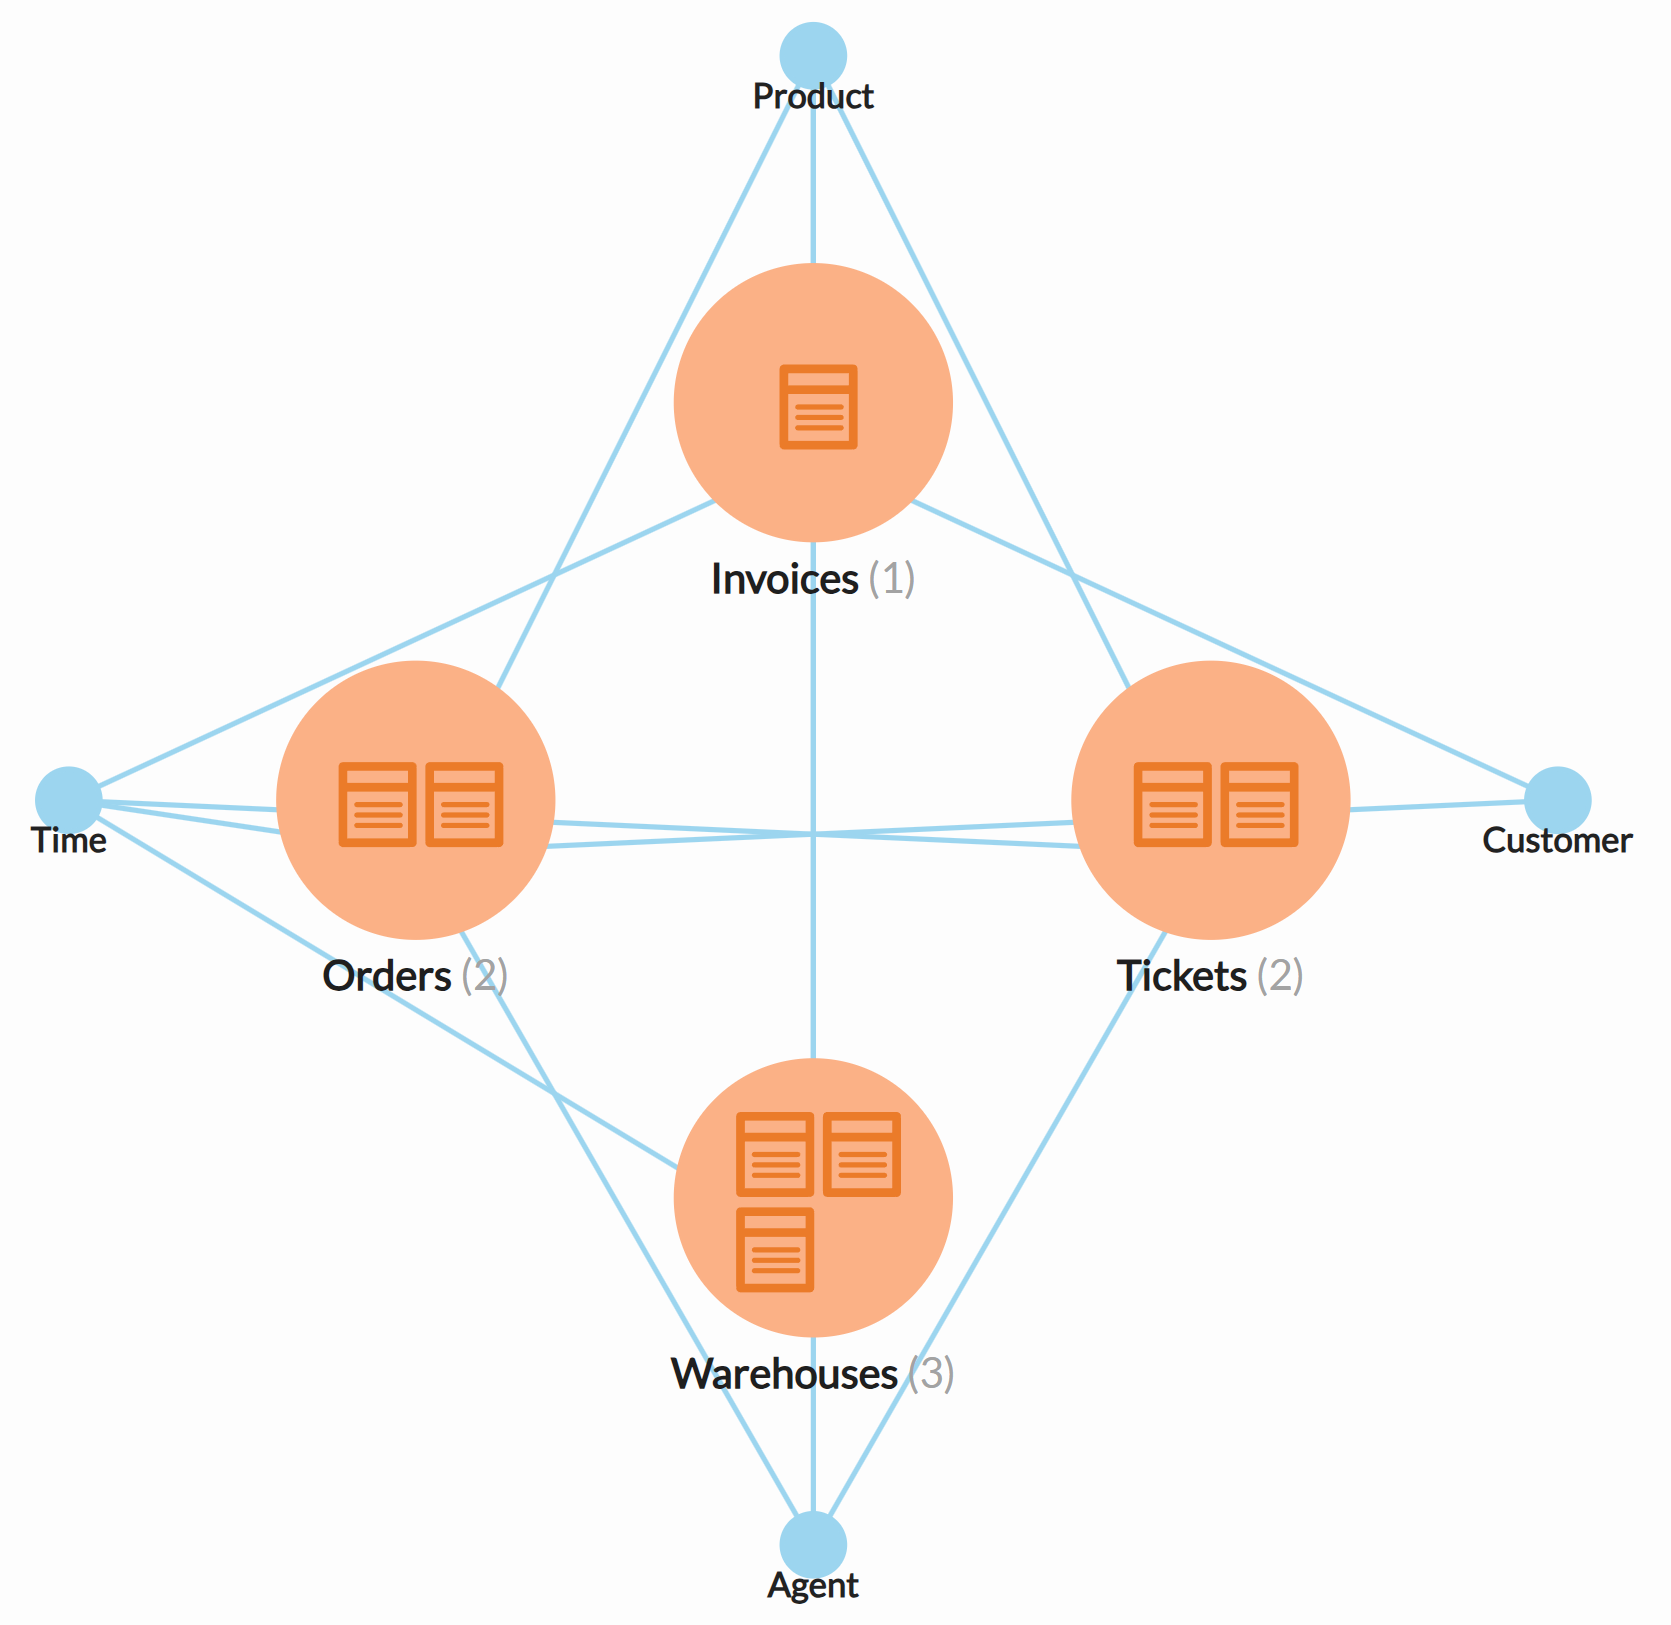
\includegraphics[width=\textwidth]{parts/methods/images/fig-indyco-dw.png}
        \caption{}
        \label{fig:llm-indyco-dw}
    \end{subfigure}
    \begin{subfigure}{0.58\linewidth}
        \centering
        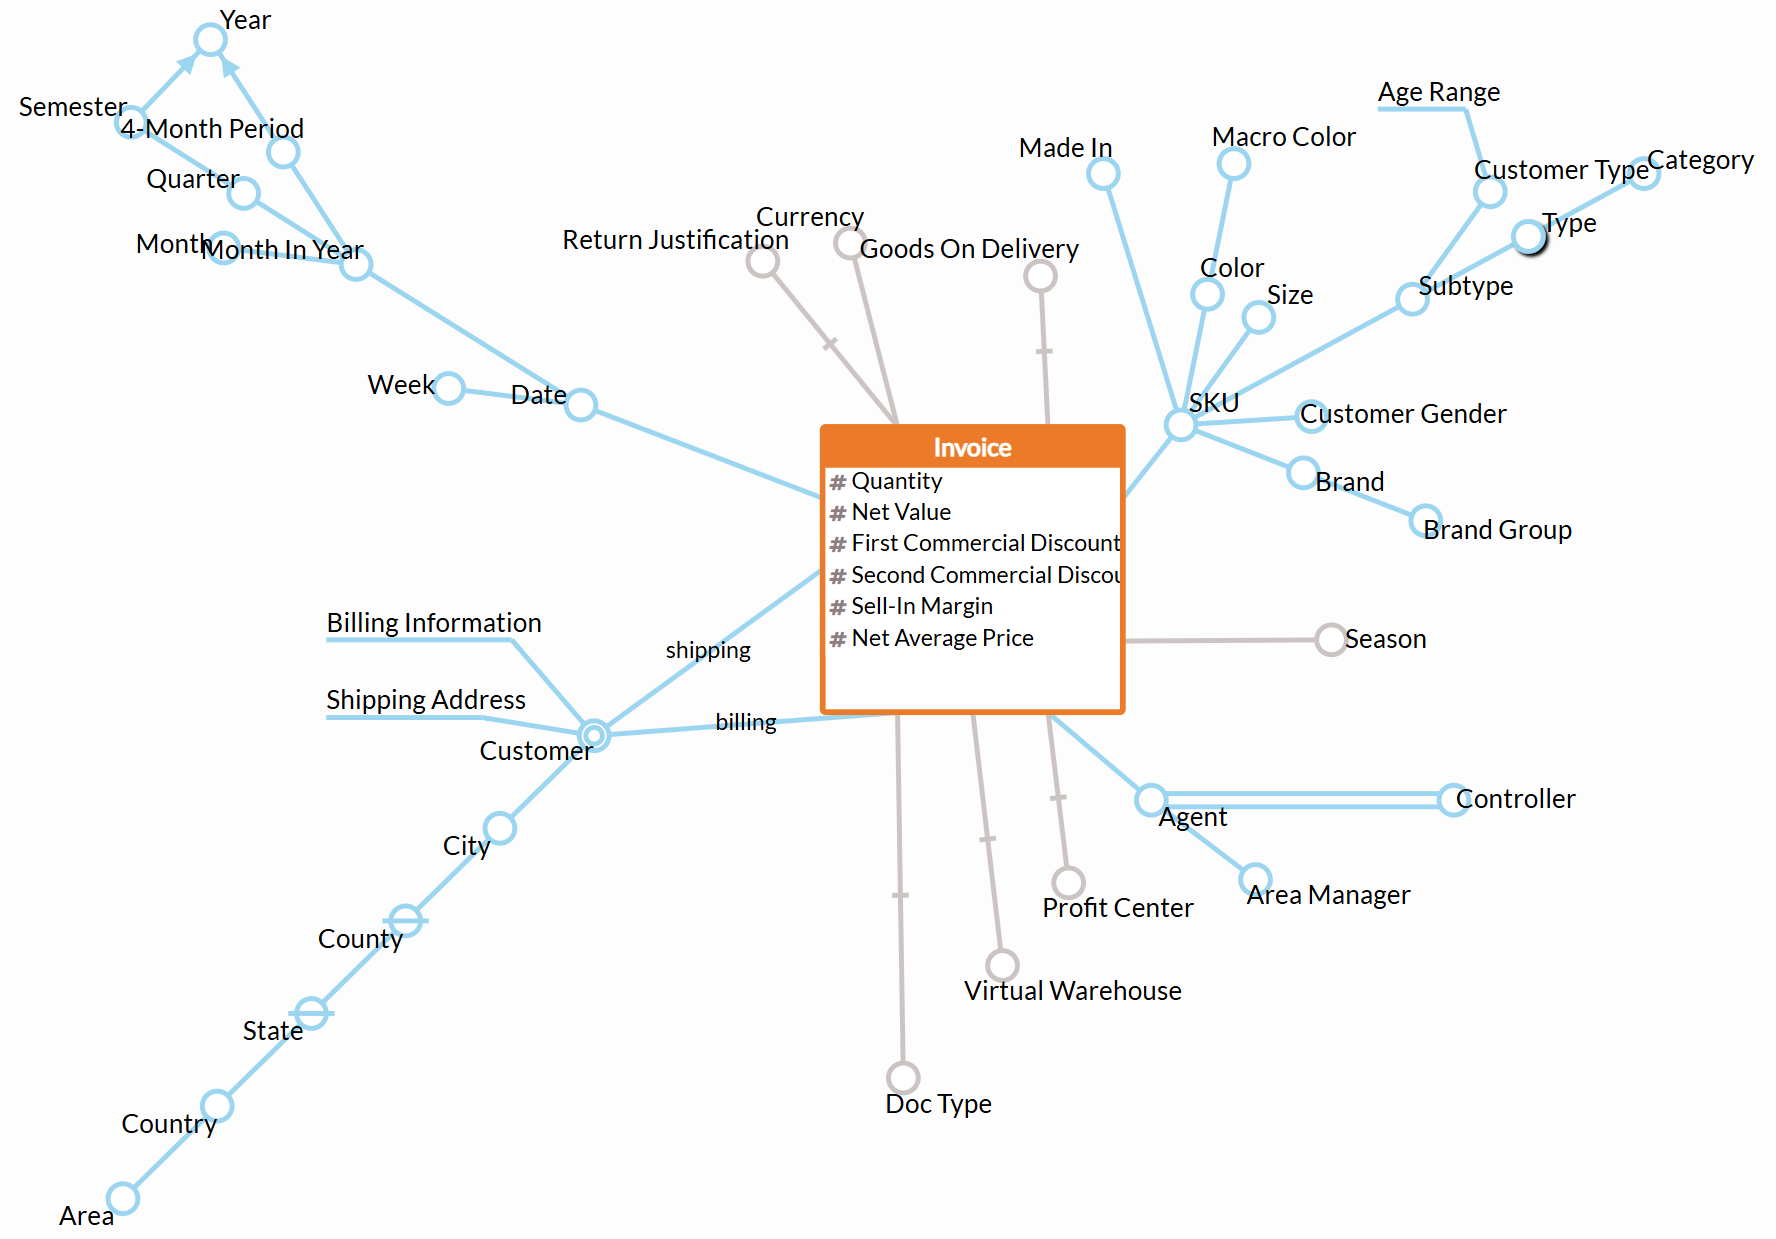
\includegraphics[width=\textwidth]{parts/methods/images/fig-indyco-dw-invoice2.png}
        \caption{}
        \label{fig:llm-indyco-dw-invoice}
    \end{subfigure}
    \caption{An overview of the sales DW schema from Indyco Explorer, showing the data marts in orange and the hierarchies they share in blue (a), and a focus on the multidimensional schema of the \sf{Invoice} fact according to the DFM (b).}
    \label{fig:llm-indyco}
\end{figure}

To model the facts in the DW, we take as a reference an advanced form of the DFM, which includes, besides the basic constructs of measure, dimension, and hierarchy, some advanced constructs such as descriptive attributes, multiple arcs, shared hierarchies, and additivity.
In this form, a fact schema is essentially a graph whose root is the \emph{fact} (depicted as a box with the fact name, e.g., \sf{Invoice} in \Cref{fig:llm-indyco-dw-invoice}, followed by a list of \emph{measures}, e.g., \sf{Quantity}), whose other nodes are \emph{attributes} (e.g., \sf{Agent}), represented as circles and connected by arcs that normally represent many-to-one \emph{roll-up relationships}, i.e., functional dependencies (for instance, $\sf{Subtype} \rightarrow \sf{Type}$). \emph{Descriptive attributes} cannot be used for aggregation and are underlined (e.g., \sf{Shipping Address}).
A \emph{multiple arc} models a many-to-many relationship between two attributes (e.g., an \sf{Agent} has multiple \sf{Controller}s) and is represented by a double arc. A \emph{shared hierarchy} is reused twice or more within the same fact (e.g., \sf{Customer} appears both as a shipping customer and a billing customer).

\begin{figure}[htbp]
    \centering
    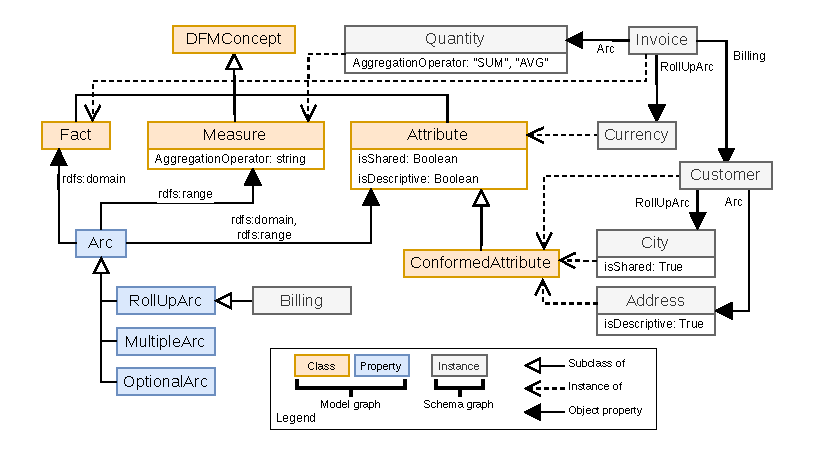
\includegraphics[width=\textwidth]{parts/methods/images/fig-onto_0-kg_0.pdf}
    \caption{A graphical representation of the KG, featuring the MG (in orange and blue) and the SG (in gray).}
    \label{fig:llm-kg}
\end{figure}

To give a formal representation of the sales DW schema, a formal representation of the multidimensional model is needed, which can then be fed to GPT. To this end, we used the RDF standard to define a KG featuring two sections that represent the multidimensional model and the DW schema, respectively (see \Cref{fig:llm-kg}):
\begin{itemize}
    \item The \textbf{Model Graph} (MG) describes the concepts that the multidimensional model relies on, and their relationships. It has been defined manually, loosely inspired by QB4OLAP \cite{DBLP:conf/dawak/EtcheverryVZ14}, and it is shown in its entirety in \Cref{fig:llm-kg}. The \textit{DFMConcept} class generalizes the main concepts of the DFM, including \textit{Fact}, \textit{Attribute}, and \textit{Measure}. An \textit{Arc} is a property that can be specialized into either \textit{RollupArc}, \textit{OptionalArc}, or \textit{MultipleArc}, representing either a (mandatory or optional) many-to-one or a many-to-many relationship between two \textit{Attributes}, respectively. A \textit{Measure} is associated with one or more \textit{AggregationOperators}. The Boolean properties \textit{isShared}, and \textit{isDescriptive} are used to refine the description of \textit{Attributes}.
    To support a DW relying on conformed hierarchies to share the same hierarchy across multiple cubes, an \textit{Attribute} can be specialized into a \textit{ConformedAttribute}.
    \item The \textbf{Schema Graph} (SG) describes a DW schema as an instance of the multidimensional model; it is automatically created by converting, via a Python script, the Excel file exported from Indyco Builder into RDF, in accordance with the MG. \Cref{fig:llm-kg} shows a small part of the SG for the sales DW, including the \sf{Invoice} fact with \sf{Quantity} as one of its measures and \sf{Currency} and \textit{Customer} as two of its dimensions. The latter includes a \textit{RollUpArc} to \sf{City} and a generic \textit{Arc} to the \sf{Address} descriptive attribute. As the customer dimension is shared by multiple facts, all its attributes are instances of \textit{Conformed Attribute}.
\end{itemize}

For the sake of the investigation, both the MG and the SG were defined in two versions: a basic one and an enriched one. The \textbf{basic} versions are those discussed above, which we will call MG$^\text{bas}$ and SG$^\text{bas}$. The \textbf{enriched} versions, namely MG$^\text{enr}$ and SG$^\text{enr}$, extend their basic counterparts with NL descriptions. In particular:
\begin{itemize}
    \item MG$^\text{enr}$ enriches every \textit{DFMConcept} and \textit{Arc} with a definition (inspired by \cite{golfarelli2009data}) and/or comments that explain what the concept represents and how it should be used. For instance, the enrichment of the \textit{RollUpArc} explains the transitivity of the arcs and how roll-up and drill-down paths should be inferred. Thus, MG$^\text{enr}$ suggests GPT how to interpret the SG from a structural perspective.
    \item SG$^\text{enr}$ enriches every instance of \textit{DFMConcept} and \textit{Arc} with a domain-oriented description (similar to a glossary) and, where applicable, a list of 20-30 sample values. These descriptions and sample values have been generated with GPT by expanding the original descriptions in Indyco Builder (which were minimal and often missing) and manually corrected/validated.
\end{itemize}

Note that the KG focuses only on the conceptual schema of the DW; this allows us to (i) maintain independence from its logical implementation, (ii) rely on business terms that are closer to NL than their logical counterparts, (iii) retain richer semantics (e.g., roll-up relationships between attributes) that would be lost in the logical schema (due to denormalization).

\subsection{Experiment Design}
\label{sec:llm-expd}

All the experiments have been conducted with OpenAI's GPT5. As a baseline for the investigation, we consider Indyco\footnote{\url{https://www.iconsulting.biz/en/indyco/}}, a CASE tool for DW design offering two distinct front-end options: \emph{Indyco Builder}, which is meant to be used by DW designers, and \emph{Indyco Explorer}, which gives business users an intuitive view of the overall information content of the DW.

The public repository \url{http://github.com/big-unibo/llm4bi} contains: (i) the MG expressed in the Turtle (TTL) serialization format, (ii) the script to convert the Indyco metadata from Excel into RDF, (iii) the SG for the sales DW in TTL format, (iv) the prompts used in the experiments, and (v) the code to run the experiments.

\subsubsection{Investigation Questions}
\label{sec:llm-rqs}

To drive the investigation, we formulated the following questions (denoted as Q1--Q3 to avoid confusion with the research questions of this thesis):
\begin{enumerate}[leftmargin=31pt,label=Q{\arabic*}:]
    \item For which types of queries on DW metadata does GPT improve over basic search?
    \item To what extent does the performance of GPT improve when the MG describing the multidimensional model is enriched with NL descriptions?
    \item To what extent does the performance of GPT improve when the SG describing the multidimensional schema is enriched with NL descriptions?
\end{enumerate}

\subsubsection{Base Criteria}
The criteria followed in the experiments are summarized below:
\begin{itemize}
    \item \textbf{Learning}.
    We couple a prompt-based learning method, which is often used as an alternative to fine-tuning \cite{DBLP:conf/models/ChenYCLMV23} with \emph{few-shot learning}, which relies on training examples in addition to the task description and input \cite{DBLP:conf/nips/BrownMRSKDNSSAA20}.

    \item \textbf{Reproducibility}. Due to their non-deterministic character, the tests' lack of reproducibility is a major obstacle when working with LLMs. The temperature parameter of GPT determines the degree of ``creativity''; as the tasks we consider do not require creativity, we set the temperature to 0 for each session.

    \item \textbf{Conversation-awareness}. The prior queries posed during a chat may have a significant impact on the responses that GPT provides. Therefore, we initiate a fresh chat for every query \cite{DBLP:journals/sosym/CamaraTBV23}. Besides, the prompts for each query are submitted 5 times to GPT in separate chats, and the results are then averaged.

    \item \textbf{Iteration}. The initial response received is taken into consideration in all of our testing.
\end{itemize}

\subsubsection{Input/output Format}
\label{sec:llm-in-out}

Both the MG and the SG are given in input to GPT for the task. Since GPT is already familiar with subject-predicate-object triples, we express the input via TTL.

To code the output, i.e., the answers returned by GPT, we adopt YAML (YAML Ain't Markup Language), a human-readable data serialization language commonly used for configuration files and in applications where data are being stored or
transmitted.\footnote{\url{https://yaml.org/spec/history/2001-08-01.html}}
The output content can vary significantly depending on the end-user query; to enable automatic parsing and evaluation of the answers, we instructed GPT to follow a specific structure based on the following tags:
\begin{itemize}
    \item \textit{Full}: a string containing the full, free-text answer.
    \item \textit{Motivation}: a string that explains the rationale for the answer.
    \item \textit{Structured}: a concise representation of the full answer, compliant with a query-specific format that falls within one of these types:
        \begin{itemize}
            \item Open-ended: A string in NL that summarizes the full answer.
            \item Close-ended: One in a set of fixed values (e.g., ``Yes'' or ``No'').
            \item Set: A set of names of facts, attributes, or measures.
            \item Set of sets: A set of sets of names, e.g., representing groups of semantically-related attributes.
            \item Set of lists: A set of lists of names, e.g., representing roll-up paths.
        \end{itemize}
\end{itemize}

\subsubsection{Query Benchmark}
\label{sec:llm-cases}

To assess the capabilities of GPT in query answering on the SG, we defined a set of 24 queries organized into four categories:
\begin{itemize}
    \item \textbf{Business queries} are aimed at describing one or more DFM concepts from a business perspective. Two examples are: \textit{``Give me a business-oriented description of the order cube''} and \textit{``Which relationship holds between brands and product categories?''}
    \item \textbf{OLAP-related queries} are aimed at determining whether a given OLAP query is supported by the DW, or how a cube can be explored via the standard OLAP operators (e.g., roll-up and drill-down). Examples are: \textit{``If I have aggregated sales data by store, which roll-up paths are available?''} and \textit{``Can I find the total quantities of shop tickets by area manager and product category?''}.
    \item \textbf{Search queries} are aimed at looking for specific DFM concepts or at discovering the relationships between them. An example is: \textit{``In which facts can I find information about customers?''}.
    \item \textbf{Test queries} are aimed at assessing the correctness of the DW schema or at refining it with missing metadata. Examples are: \textit{``Are there multiple measures with different names but same semantics?''} and \textit{``Are there measures whose business meaning implies they should be non-additive, while their aggregation operators include SUM?''}.
\end{itemize}

When applicable, queries are formulated in two versions: a \textit{clean} version that precisely refers to DFM concepts with the names they have in the MG, and a \textit{dirty} version that uses synonyms.

\subsubsection{Prompt Templates}
\label{sec:llm-templates}

Following the suggestions given in \cite{DBLP:journals/corr/abs-2305-12138}, the prompts adopted in Q2 and Q3 to formulate the queries submitted to GPT are structured according to the following template:
\begin{enumerate}
        \item ROLE: the specific roles assigned to GPT and to the user to provide a context for the task:
            \begin{shaded} \scriptsize \noindent
                \textbf{Prompt}: You are an expert in Business Intelligence and Data Warehousing. I am the end-user.
            \end{shaded}
        \item INPUT: the MG and the SG over which the queries will be asked:
            \begin{shaded} \scriptsize \noindent
                \textbf{Prompt}: The following is an ontology in Turtle format representing the Dimensional Fact Model: \textcolor{blue}{[MG in TTL]}. Below you can find (in the form of Turtle triples) the DFM schema of a set of OLAP cubes, described through the above ontology: \textcolor{blue}{[SG in TTL]}
            \end{shaded}
        \item TASK: the query to be asked:
            \begin{shaded} \scriptsize \noindent
                \textbf{Prompt}: Now I am going to ask a question about the metadata of these cubes: \textcolor{blue}{[Question text]}
            \end{shaded}
        \item FORMAT: how the output should be coded:
            \begin{shaded}
                \scriptsize \noindent
                \textbf{Prompt (excerpt)}: I expect you to provide the following output. (1) The full answer you would give to the query.
                (2) A concise, structured version of the answer that strictly follows the following format instructions: \textcolor{blue}{[Query-specific required format]}
                (3) A concise explanation of how you derived the answer, mentioning the key elements that led to it.
            \end{shaded}
        \item EXAMPLES: a list of 12 examples, comprising the text of the query and the expected answer in the above format.
\end{enumerate}

\subsubsection{Evaluation of the Results}
\label{sec:llm-metrics}

Q2 and Q3 require a quantitative assessment of the accuracy of the structured part of each answer given by GPT, $A$, with reference to a ground truth $T$ defined by expert users. Given the variety of queries and of the corresponding output formats, the \textbf{accuracy} is determined using different methods, all returning a value $v \in [0,1]$, where 1 represents a perfect answer.
\begin{itemize}
    \item Open-ended: $v$ is returned by GPT itself, using an ad-hoc prompt asking to evaluate to what extent $A$ reflects $T$ (a.k.a. \textit{LLM-as-a-judge} \cite{gu2024survey}).
    \item Close ended: $v=1$ if $A=T$, $v=0$ otherwise.
    \item Set: $v$ is computed as the F1-Score of $A$.
    \item Set of sets: $v$ is computed as the Constrained Entity-Alignment F1-Score (CEAF-F1) \cite{luo2005coreference}, which essentially finds the F1-Score of the best one-to-one alignment between the sets in $A$ and those in $T$. Alignments are scored using the Jaccard similarity.
    \item Set of lists: $v$ is computed using CEAF-F1, where the alignments are scored via the ROUGE-L similarity, which builds on the Longest Common Subsequence (LCS) between the compared lists.
\end{itemize}
Except for open-ended queries, simple methods for entity matching between strings are implemented (e.g., replacing upper-case letters with lower-case ones).

\subsection{Experiments and Answers to the Investigation Questions}
\label{sec:llm-exp}

\subsubsection{Q1}

To answer this question we consider the four categories of queries introduced in \Cref{sec:llm-cases}. Besides, we refer to four main types of end-users:
\begin{itemize}
    \item \emph{naive user}, who only has shallow knowledge of the business domain and of the basic constructs of the DFM (namely, fact, measure, and dimension);
    \item \emph{business user}, who knows the basic constructs of the DFM but has deep knowledge of the business domain;
    \item \emph{technical user}, who has shallow knowledge of the business domain but is knowledgeable in the advanced constructs of the DFM (e.g., additivity and complex hierarchies);
    \item \emph{smart user}, who has deep knowledge of both the business domain and the DFM.
\end{itemize}
We assume for simplicity that all these users know the OLAP operators.

As already mentioned, as a baseline we use the querying capabilities offered by Indyco, and specifically by its Explorer, which delivers an intuitive and complete view of the information content of a DW oriented to business users. The DW metadata managed by Indyco Explorer include the complete DFM schemata of the facts in the DW, including conformed dimensions, plus a glossary that associates each DFM concept with additional information such as its description and some sample values. To navigate these metadata, the tool offers the possibility to view DFM diagrams at different levels of detail, as shown in \Cref{fig:llm-indyco-dw}. Besides, all metadata can be searched (relying on exact name matches).

We start by considering the first category of queries, i.e., business queries. An example is ``Give me a business-oriented description of the invoice cube''. Clearly, answering this query with Indyco would entail (i) opening the page that visualizes the DFM schema for the \sf{Order} cube; (ii) interpreting the formalism to infer the role of the different concepts and their relationships; and (iii) elaborating on the result and organizing it into a clear and precise text. Clearly, step (ii) is completely out of reach for naive and business users; even for technical and smart users, it would require a significant effort and time. We also note that, if the user is technical, (s)he may not know the \emph{exact} fact name, which would make Indyco search unfruitful (e.g., (s)he might look for ``bills'' instead of ``order'').

As to OLAP-related queries (e.g., ``Can I find the total quantities of shop tickets by area manager and product category?''), they definitely require deep knowledge of the DFM to be answered. If the exact names of concepts are not known (e.g., ``Can I compute the average quantities of DOS stores sales by agent coordinators and product classifications?''), they also require good knowledge of the business domain. Thus, these queries are within smart users' reach only; they can be answered on Indyco by (i) searching the fact to which the required measure(s) belong; (ii) opening the DFM schema for that fact; and (iii) checking that the required aggregation levels are part of the hierarchies.

Search queries are mostly answered with some basic knowledge of the DFM, via one or more Indyco searches. For instance, ``Which facts can be analyzed by SKU (Stock Keeping Unit) and store together?'' can be answered by (i) searching for ``SKU''; (ii) searching for ``store''; and (iii) finding the facts that belong to the results of both searches.
However, since they require knowing the exact concept names, they are more easily answered by business and smart users.

Finally, test queries require designer-level knowledge of the DFM. Considering that they often involve synonym checking, they can be answered by smart users only, and with a significant effort.

When GPT is used instead of Indyco, all end-user types have the same possibilities since NL is used for query formulation. In particular, several benchmark queries are \emph{dirty}, i.e., they do not use the exact names of DFM concepts but their synonyms; this allows us to cover users with little knowledge of the application domain as well.
The accuracy obtained when answering the queries in the benchmark with GPT using the basic versions of the KG (MG$^\text{bas}$ and SG$^\text{bas}$) is shown in \Cref{fig:llm-f1-queries}. Prime queries are the dirty ones, i.e., the ones that do not use the exact names of DFM concepts but their synonyms
(e.g., $q'_3$ is the dirty version of $q_3$). It turns out that search queries yield the best accuracy (0.94 on average). OLAP-related queries yield good accuracy, although several queries asking for the feasibility of a given OLAP query are given the wrong answer. The unsatisfactory results obtained with business queries can be explained considering that all four queries giving an accuracy of 0 ask for the multiplicity of the relationship between two hierarchy attributes (typically, either many-to-one or many-to-many); since GPT has not been taught how to infer this, it gives a wrong answer in most cases. The category with the worst accuracy is test queries, with only 0.39 average accuracy; this is not surprising because of the inherent complexity of the task, especially when reasoning with additivity.

\begin{figure}[htbp]
    \centering
    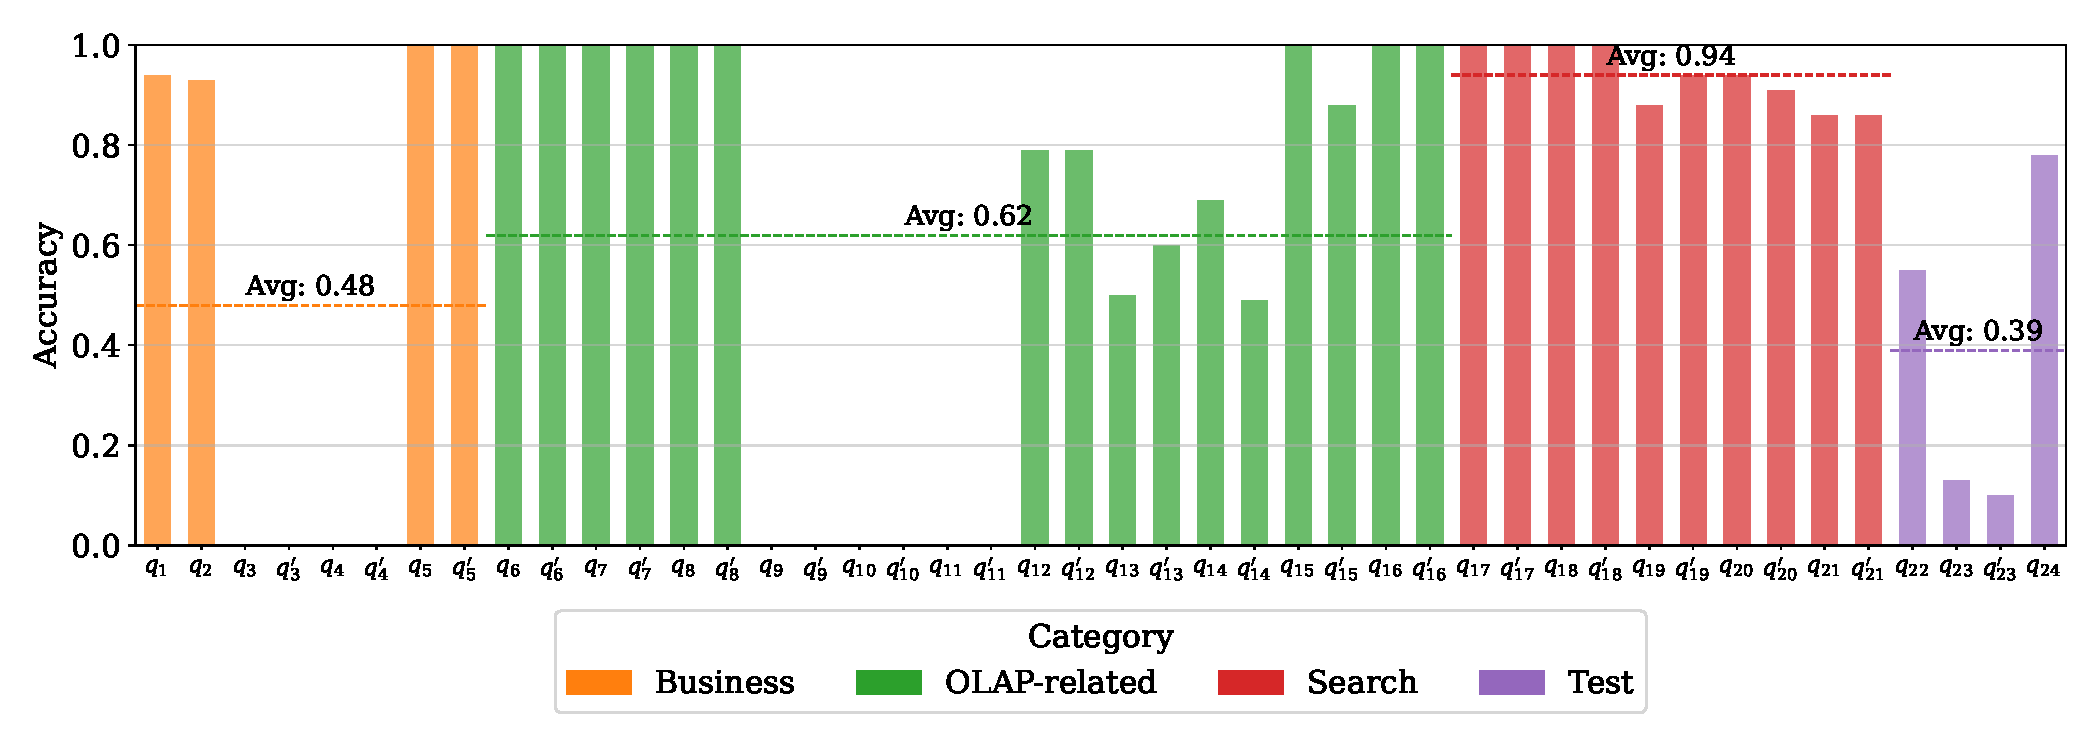
\includegraphics[width=\textwidth]{parts/methods/images/fig-f1_queries.pdf}
    \caption{Accuracy in metadata query answering by GPT using the basic versions of the KG; dashed lines show the average accuracy for each query category.}
    \label{fig:llm-f1-queries}
\end{figure}

Based on the above, Q1 can be answered as follows: ``GPT improves over basic search by making all queries available to all user types with small effort. However, while search queries are answered with high accuracy, for the other types of queries the accuracy is not fully satisfactory''.

\subsubsection{Q2 and Q3}

The results shown in \Cref{fig:llm-f1-queries} leave a large space for improvement. These questions aim at understanding if this is possible by enriching the KG with explanations, descriptions, and how-to suggestions. To this end, we made two additional rounds of experiments: one where MG$^\text{enr}$ is fed to GPT instead of MG$^\text{bas}$, and one where SG$^\text{bas}$ is also replaced with SG$^\text{enr}$.
\Cref{fig:llm-f1-all} shows the average accuracy in answering the benchmark queries per query category and overall. At first glance, enhancing the MG appears to be the most rewarding activity, as the overall accuracy only slightly increases with SG$^\text{enr}$. However, a closer look at the results reveals the following:

\begin{figure}[htbp]
    \centering
    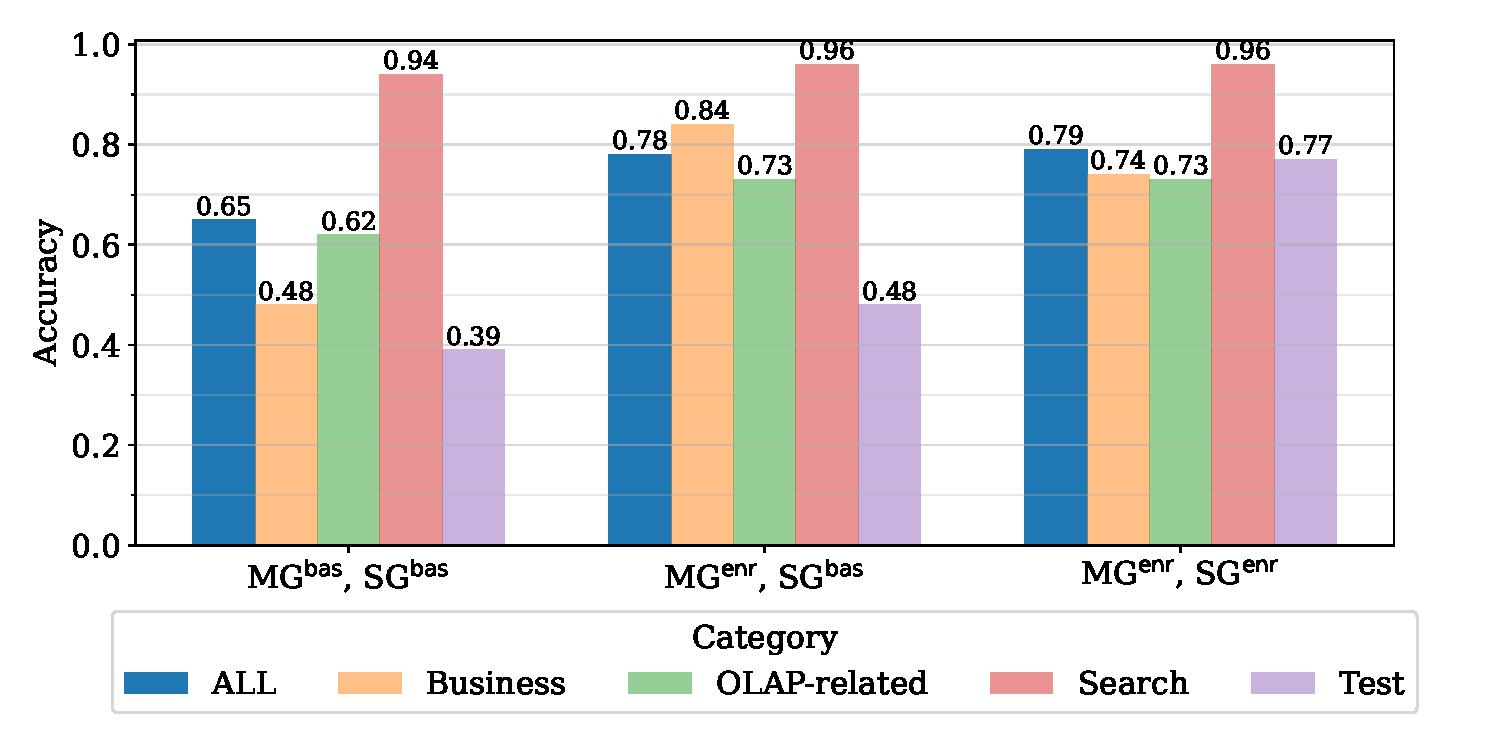
\includegraphics[width=0.8\textwidth]{parts/methods/images/fig-f1_all.pdf}
    \caption{Average accuracy in metadata query answering by GPT using the enriched versions of the KG.}
    \label{fig:llm-f1-all}
\end{figure}

\begin{itemize}
    \item Enhancing the MG improves the accuracy for the queries where the problem was due to a misinterpretation of the direction and semantics of \textit{Arcs} (e.g., wrongly assuming that a multiple arc implies a many-to-one relationship).
    \item Enhancing the SG improves the accuracy of the answers that require a deeper and broader reasoning on the semantics of the concepts in the DW schema (in particular for test queries, which require a comparison of multiple concepts in the KG). However, it can also induce hallucinations on queries focused on concepts with overlapping meaning; for instance, GPT confuses the categorization of brands with the categorization of products, so it suggests a roll-up from \sf{Brand} to the product's \sf{Category}, although they actually are on different branches of the \sf{SKU} hierarchy.
    \item While business queries failed to provide sufficient accuracy with the basic versions of the KG, their accuracy doubles when the graph is enriched with NL explanations. Interestingly, this is the only category whose accuracy decreases after enhancing the SG as well. This is due to a single query ($q_3$, asking ``Which relationship holds between brands and product categories?''), which experiences the above-mentioned hallucination problem.
    \item The accuracy of OLAP-related queries increases with MG$^\text{enr}$ and is not affected by SG$^\text{enr}$. This is not surprising, as these queries are more focused on DFM and OLAP than on the business domain.
    \item Search queries already show an almost-optimal accuracy in the basic setting, thus they are not significantly affected by enhancements.
    \item The most significant improvement that comes with SG$^\text{enr}$ is for test queries. Indeed, these queries require a deeper reasoning on the semantics of the DFM concepts, thus the NL descriptions added in SG$^\text{enr}$ help a lot with answering.
\end{itemize}

Based on the above, Q2 and Q3 can be concisely answered as follows: ``The overall accuracy of GPT improves by 0.13 when the MG is enriched, and by 0.01 when the SG is enriched''.

\subsection{Conclusion and Future Directions}
\label{sec:llm-concl}

This section explored the capabilities of LLMs, in particular of GPT, in answering queries on DW metadata. As a baseline, we considered the search and exploration capabilities offered by Indyco, a CASE tool specifically devised for DW design. The experiments show that the use of GPT has several advantages: (i) GPT provides end-users with an NL interface, which allows them to formulate queries in a non-technical way and relieves them from the tedious task of searching metadata and interpreting the diagrams; (ii) it returns a motivated result in NL, which makes metadata search within the reach of users of all kinds, independently of their technical and business knowledge; (iii) it is tolerant to the use of synonyms, which allows users to find a result even if they do not recall the exact name of a concept in the DW; (iv) it can quickly tell users if a given analysis they have in mind is actually feasible; (v) it can help in highlighting anomalies in the DW schema, due for instance to a wrong setting of aggregation operators or to duplicate concepts.

Despite these encouraging preliminary results, several aspects still need to be investigated to overcome the limitations encountered, particularly with regard to hallucinations, which persist even after KG enrichments. First, moving from a single-agent to a multi-agent approach would allow each agent to specialize in a specific category (or subcategory) of queries, with dedicated prompts and examples. Second, neuro-symbolic techniques combining the reasoning capabilities of the LLM with Cypher-like queries to the KG can help reduce the hallucination phenomenon. Third, a RAG-based approach can restrict the context provided to the LLM to the relevant portion of the KG, with the dual advantage of increasing the focus and reducing the length (thus, the cost) of each prompt. Further future work includes the extension of the experimental evaluation by broadening the query benchmark and by analyzing the impact of the enrichments on the different user categories.
